% Exam Template for UMTYMP and Math Department courses
%
% Using Philip Hirschhorn's exam.cls: http://www-math.mit.edu/~psh/#ExamCls
%
% run pdflatex on a finished exam at least three times to do the grading table on front page.
%
%%%%%%%%%%%%%%%%%%%%%%%%%%%%%%%%%%%%%%%%%%%%%%%%%%%%%%%%%%%%%%%%%%%%%%%%%%%%%%%%%%%%%%%%%%%%%%

% These lines can probably stay unchanged, although you can remove the last
% two packages if you're not making pictures with tikz.
\documentclass[11pt]{exam}
\RequirePackage{amssymb, amsfonts, amsmath, latexsym, verbatim, xspace, setspace, graphicx}


% By default LaTeX uses large margins.  This doesn't work well on exams; problems
% end up in the "middle" of the page, reducing the amount of space for students
% to work on them.
\usepackage[margin=1in]{geometry}
\usepackage[english]{babel}
\usepackage[autostyle]{csquotes} %%%% This package allows Tex to recognize quotation marks with the \enquote command. 


% Here's where you edit the Class, Exam, Date, etc.
\newcommand{\class}{MAT 203}
\newcommand{\term}{Summer I 2020}
\newcommand{\examnum}{Final Exam}
\newcommand{\examdate}{06/29/20}
\newcommand{\timelimit}{3 hours and 25 minutes}

% For an exam, single spacing is most appropriate
\singlespacing
% \onehalfspacing
% \doublespacing

% For an exam, we generally want to turn off paragraph indentation
\parindent 0ex
\title{MAT 203 - Summer I 2020: Final practice}
\begin{document} 

% These commands set up the running header on the top of the exam pages
\pagestyle{head}
\firstpageheader{}{}{}\textbf{}
\runningheader{\class}{\examnum\ - Page \thepage\ of \numpages}{\examdate}
\runningheadrule

\begin{flushright}
\begin{tabular}{p{2.8in} r l}
\textbf{\class} & \textbf{Name (Print):} & \makebox[2in]{\hrulefill}\\
\textbf{\term} &&\\
\textbf{\examnum} &&\\
\textbf{\examdate} &&\\
\textbf{Time Limit: \timelimit} & ID number & \makebox[2in]{\hrulefill}
\end{tabular}\\
\end{flushright}
\rule[1ex]{\textwidth}{.1pt}

\begin{center}
\large{\textbf{Instructions}}
\end{center}

\begin{minipage}[t]{3.7in}
\vspace{0pt}
\begin{itemize}

\item This exam contains \numpages\ pages (including this cover page) and
\numquestions\ problems.  Check to see if any pages are missing.  Enter
all requested information on the top of this page, and put your initials
on the top of every page, in case the pages become separated.

\item This is an open-book exam. You may not use a calculator.

\item \textbf{Organize your work}, in a reasonably neat and coherent way, in
the space provided. Work scattered all over the page without a clear ordering will 
receive very little credit.  

\item \textbf{Mysterious or unsupported answers will not receive full
credit}.

\end{itemize}

\end{minipage}
\hfill
\begin{minipage}[t]{2.3in}
\vspace{0pt}
%\cellwidth{3em}
\gradetablestretch{2}
\vqword{Problem}
\addpoints % required here by exam.cls, even though questions haven't started yet.	
\gradetable[v]%[pages]  % Use [pages] to have grading table by page instead of question

\end{minipage}
\newpage % End of cover page

%%%%%%%%%%%%%%%%%%%%%%%%%%%%%%%%%%%%%%%%%%%%%%%%%%%%%%%%%%%%%%%%%%%%%%%%%%%%%%%%%%%%%
%
% See http://www-math.mit.edu/~psh/#ExamCls for full documentation, but the questions
% below give an idea of how to write questions [with parts] and have the points
% tracked automatically on the cover page.
%
%
%%%%%%%%%%%%%%%%%%%%%%%%%%%%%%%%%%%%%%%%%%%%%%%%%%%%%%%%%%%%%%%%%%%%%%%%%%%%%%%%%%%%%

\begin{questions}

% Basic question
%%%%%%%%%%%%%%

\addpoints
\question A heated storage room is to be constructed in the shape of a rectangular prism, with total volume $1000 \mathrm{ft}^3$. The floor is to be insulated so that the heat loss though it may be considered as $0$. Because warm air rises, the heat loss per unit of area through the ceiling is twice as great as the heat loss through the lateral walls.
\begin{parts}
\part[3] Sketch the room, labeling the dimensions of its sides. Describe the heat loss function according to your sketch. 
\vfill
\part[3] Use the volume constraint to reduce the number of variables in the heat loss function to two. 
\vfill
\part[4] Compute the gradient of the symplified heat loss function found on part (b). 
\vfill
\newpage
\part[5] Find the critical points of the heat loss function. 
\vfill
\part[5] Use the Second Partials Test to determine which critical point, if any, minimizes heat loss. 
\vfill
\end{parts}

\newpage 


%%%%%%%%%%%%%%%%%%%%%%%%%%%%%%%%%%%
\addpoints 
\question The table below contains a collection of data points.
\begin{center}
\begin{tabular}{|c|c|c|c|c|c|c|}
\hline 
x & 0 & 2 & 4 & 7 & 9 & 12\\ 
\hline 
y & 10 & 8 & 7 & 5 & 3 & 0\\ 
\hline 
\end{tabular} 
\end{center}

\begin{parts}
\part[5] Given a line with equation $y=ax+b$, describe a function, in terms of the variables $a$ and $b$, measuring the sum of the square-distances between the points in the table above and the points with corresponding $x$-coordinate on the line.
\vfill
\part[5] Find the gradient of the function you described in part (a). 
\vfill
\newpage
\part[5] Find the critical points of the function you described in part (a).
\vfill
\part[5] Find the equation of the regression line approximating the points in the table by determining which of the critical points you found on part (c), is a minimum. 
\vfill
\end{parts}

\newpage

%%%%%%%%%%%%%%%%%
\addpoints
\question This problem concerns the iterated integral
\begin{equation*}
\int_{0}^{1} \int_{y}^{1} sin(x^2) \, dx \, dy.
\end{equation*}

\begin{parts}
\part[5] Sketch the region of integration in the plane.
\vfill 
\part[5] Switch the order of integration.
\vfill
\newpage
\part[10] Evaluate the integral by using whichever order you prefer. 
\vfill
\end{parts}
\newpage
%%%%%%%%%%%%%%%%%%%%
\addpoints
\question[10] Use polar coordinates to find the area between inside the circle with equation $r=2$ and outside the rose curve with equation 
\begin{equation*}
r = |\cos(2\theta)|
\end{equation*}
\newpage 
%%%%%%%%%%%%%%%%%%%

\addpoints
\question This problem concerns the iterated integral
\begin{equation*}
\int_{0}^{3} \int_{0}^{\sqrt{9-x^2}} \int_{0}^{\sqrt{9-x^2-y^2}} \sqrt{x^2+y^2+z^2} \, dz \, dy \, dx.
\end{equation*}
Below is a plot of the region of integration, for your convenience.
\begin{center}
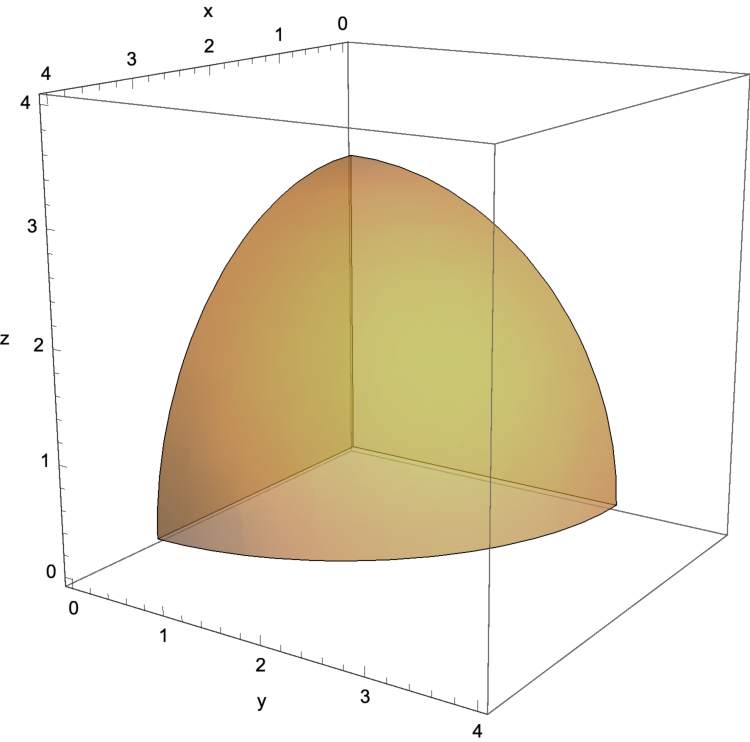
\includegraphics[scale=0.5]{p5.pdf}
\end{center}
\begin{parts}
\part[8] Convert it to cylindrical coordinates (do not evaluate).
\vfill
\part[8] Convert it to spherical coordinates (do not evaluate).
\vfill
\newpage
\part[14] Evaluate the integral by using your preferred system of coordinates: Cartesian, cylindrical, or spherical. 
\vfill
\end{parts}
%%%%%%%%%%%%%%%%%%%%%%%%%%

\end{questions}
\end{document}
